%%%%% Set up %%%%%

% Set document style and font size
\documentclass[12pt]{article}\usepackage[]{graphicx}\usepackage[]{color}
%% maxwidth is the original width if it is less than linewidth
%% otherwise use linewidth (to make sure the graphics do not exceed the margin)
\makeatletter
\def\maxwidth{ %
  \ifdim\Gin@nat@width>\linewidth
    \linewidth
  \else
    \Gin@nat@width
  \fi
}
\makeatother

\definecolor{fgcolor}{rgb}{0.345, 0.345, 0.345}
\newcommand{\hlnum}[1]{\textcolor[rgb]{0.686,0.059,0.569}{#1}}%
\newcommand{\hlstr}[1]{\textcolor[rgb]{0.192,0.494,0.8}{#1}}%
\newcommand{\hlcom}[1]{\textcolor[rgb]{0.678,0.584,0.686}{\textit{#1}}}%
\newcommand{\hlopt}[1]{\textcolor[rgb]{0,0,0}{#1}}%
\newcommand{\hlstd}[1]{\textcolor[rgb]{0.345,0.345,0.345}{#1}}%
\newcommand{\hlkwa}[1]{\textcolor[rgb]{0.161,0.373,0.58}{\textbf{#1}}}%
\newcommand{\hlkwb}[1]{\textcolor[rgb]{0.69,0.353,0.396}{#1}}%
\newcommand{\hlkwc}[1]{\textcolor[rgb]{0.333,0.667,0.333}{#1}}%
\newcommand{\hlkwd}[1]{\textcolor[rgb]{0.737,0.353,0.396}{\textbf{#1}}}%
\let\hlipl\hlkwb

\usepackage{framed}
\makeatletter
\newenvironment{kframe}{%
 \def\at@end@of@kframe{}%
 \ifinner\ifhmode%
  \def\at@end@of@kframe{\end{minipage}}%
  \begin{minipage}{\columnwidth}%
 \fi\fi%
 \def\FrameCommand##1{\hskip\@totalleftmargin \hskip-\fboxsep
 \colorbox{shadecolor}{##1}\hskip-\fboxsep
     % There is no \\@totalrightmargin, so:
     \hskip-\linewidth \hskip-\@totalleftmargin \hskip\columnwidth}%
 \MakeFramed {\advance\hsize-\width
   \@totalleftmargin\z@ \linewidth\hsize
   \@setminipage}}%
 {\par\unskip\endMakeFramed%
 \at@end@of@kframe}
\makeatother

\definecolor{shadecolor}{rgb}{.97, .97, .97}
\definecolor{messagecolor}{rgb}{0, 0, 0}
\definecolor{warningcolor}{rgb}{1, 0, 1}
\definecolor{errorcolor}{rgb}{1, 0, 0}
\newenvironment{knitrout}{}{} % an empty environment to be redefined in TeX

\usepackage{alltt}

% File path to resources (style file etc)
\newcommand{\locRepo}{csas-style}

% Style file for DFO Technical Reports
\usepackage{\locRepo/tech-report}

% header-includes from R markdown entry
\usepackage{float}

%%%%% Variables %%%%%

% New definitions: Title, year, report number, authors
% Protect lower case words (i.e., species names) in \Addlcwords{}, in "TechReport.sty"
\newcommand{\trTitle}{Quantifying shoreline modifications adjacent to eelgrass meadows in the Strait of Georgia Bioregion}
\newcommand{\trYear}{2022}
\newcommand{\trReportNum}{nnn}
% Optional
\newcommand{\trAuthFootA}{Email: \link{mailto:John.Cristiani@dfo-mpo.gc.ca}{\nolinkurl{John.Cristiani@dfo-mpo.gc.ca}} \textbar{} telephone: (250) 756-5555}
\newcommand{\trAuthsLong}{John M. Cristiani\textsuperscript{1} Katherine H. Bannar-Martin\textsuperscript{2} and Emily M. Rubidge\textsuperscript{2}}
\newcommand{\trAuthsBack}{Cristiani, J.C., Bannar-Martin, K.H, and Rubidge, E.M.}

% New definition: Address
\newcommand{\trAddy}{\textsuperscript{1}Pacific Biological Station\\
Fisheries and Oceans Canada, 3190 Hammond Bay Road\\
Nanaimo, British Columbia, V9T 6N7, Canada\\
\textsuperscript{2}Institute of Ocean Sciences\\
Fisheries and Oceans Canada, 9860 W Saanich Road\\
Sidney, British Columbia, V8L 4B2, Canada\\}

% Abstract
\newcommand{\trAbstract}{Here is the abstract text. Lorem ipsum dolor sit amet, consectetur adipisicing elit, sed do eiusmod tempor incididunt ut labore et dolore magna aliqua. Ut enim ad minim veniam, quis nostrud exercitation ullamco laboris nisi ut aliquip ex ea commodo consequat. Duis aute irure dolor in reprehenderit in voluptate velit esse cillum dolore eu fugiat nulla pariatur. Excepteur sint occaecat cupidatat non proident, sunt in culpa qui officia deserunt mollit anim id est laborum.}

% Resume (i.e., French abstract)
\newcommand{\trResume}{Voici le résumé. Lorem ipsum dolor sit amet, consectetur adipisicing elit, sed do eiusmod tempor incididunt ut labore et dolore magna aliqua. Ut enim ad minim veniam, quis nostrud exercitation ullamco laboris nisi ut aliquip ex ea commodo consequat. Duis aute irure dolor in reprehenderit in voluptate velit esse cillum dolore eu fugiat nulla pariatur. Excepteur sint occaecat cupidatat non proident, sunt in culpa qui officia deserunt mollit anim id est laborum.}

\newcommand{\trISBN}{}

\DeclareGraphicsExtensions{.png,.pdf}
%%%%% Start %%%%%

% Start the document
\IfFileExists{upquote.sty}{\usepackage{upquote}}{}

% commands and environments needed by pandoc snippets
% extracted from the output of `pandoc -s`
%% Make R markdown code chunks work
\usepackage{array}
\usepackage{amssymb,amsmath}
\usepackage{color}
\usepackage{fancyvrb}

% From default template:
\newcommand{\VerbBar}{|}
\newcommand{\VERB}{\Verb[commandchars=\\\{\}]}
\DefineVerbatimEnvironment{Highlighting}{Verbatim}{commandchars=\\\{\},formatcom=\color[rgb]{0.00,0.00,0.00}}
\usepackage{framed}
\definecolor{shadecolor}{RGB}{248,248,248}
\newenvironment{Shaded}{\begin{snugshade}}{\end{snugshade}}
\newcommand{\AlertTok}[1]{\textcolor[rgb]{0.94,0.16,0.16}{#1}}
\newcommand{\AnnotationTok}[1]{\textcolor[rgb]{0.56,0.35,0.01}{\textbf{\textit{#1}}}}
\newcommand{\AttributeTok}[1]{\textcolor[rgb]{0.77,0.63,0.00}{#1}}
\newcommand{\BaseNTok}[1]{\textcolor[rgb]{0.00,0.00,0.81}{#1}}
\newcommand{\BuiltInTok}[1]{#1}
\newcommand{\CharTok}[1]{\textcolor[rgb]{0.31,0.60,0.02}{#1}}
\newcommand{\CommentTok}[1]{\textcolor[rgb]{0.56,0.35,0.01}{\textbf{#1}}}
\newcommand{\CommentVarTok}[1]{\textcolor[rgb]{0.56,0.35,0.01}{\textbf{\textit{#1}}}}
\newcommand{\ConstantTok}[1]{\textcolor[rgb]{0.00,0.00,0.00}{#1}}
\newcommand{\ControlFlowTok}[1]{\textcolor[rgb]{0.13,0.29,0.53}{\textit{#1}}}
\newcommand{\DataTypeTok}[1]{\textcolor[rgb]{0.13,0.29,0.53}{#1}}
\newcommand{\DecValTok}[1]{\textcolor[rgb]{0.00,0.00,0.81}{#1}}
\newcommand{\DocumentationTok}[1]{\textcolor[rgb]{0.56,0.35,0.01}{\textbf{\textit{#1}}}}
\newcommand{\ErrorTok}[1]{\textcolor[rgb]{0.64,0.00,0.00}{\textit{#1}}}
\newcommand{\ExtensionTok}[1]{#1}
\newcommand{\FloatTok}[1]{\textcolor[rgb]{0.00,0.00,0.81}{#1}}
\newcommand{\FunctionTok}[1]{\textcolor[rgb]{0.00,0.00,0.00}{#1}}
\newcommand{\ImportTok}[1]{#1}
\newcommand{\InformationTok}[1]{\textcolor[rgb]{0.56,0.35,0.01}{\textbf{\textit{#1}}}}
\newcommand{\KeywordTok}[1]{\textcolor[rgb]{0.13,0.29,0.53}{\textit{#1}}}
\newcommand{\NormalTok}[1]{#1}
\newcommand{\OperatorTok}[1]{\textcolor[rgb]{0.81,0.36,0.00}{\textit{#1}}}
\newcommand{\OtherTok}[1]{\textcolor[rgb]{0.56,0.35,0.01}{#1}}
\newcommand{\PreprocessorTok}[1]{\textcolor[rgb]{0.56,0.35,0.01}{\textbf{#1}}}
\newcommand{\RegionMarkerTok}[1]{#1}
\newcommand{\SpecialCharTok}[1]{\textcolor[rgb]{0.00,0.00,0.00}{#1}}
\newcommand{\SpecialStringTok}[1]{\textcolor[rgb]{0.31,0.60,0.02}{#1}}
\newcommand{\StringTok}[1]{\textcolor[rgb]{0.31,0.60,0.02}{#1}}
\newcommand{\VariableTok}[1]{\textcolor[rgb]{0.00,0.00,0.00}{#1}}
\newcommand{\VerbatimStringTok}[1]{\textcolor[rgb]{0.31,0.60,0.02}{#1}}
\newcommand{\WarningTok}[1]{\textcolor[rgb]{0.56,0.35,0.01}{\textbf{\textit{#1}}}}
\begin{document}

%%%% Front matter %%%%%

% Add the first few pages
\frontmatter

%%%%% Drafts %%%%%

%\linenumbers  % Line numbers
%\onehalfspacing  % Extra space between lines
\renewcommand{\headrulewidth}{0.5pt}  % Header line
\renewcommand{\footrulewidth}{0.5pt}  % footer line
%\pagestyle{fancy}\fancyhead[c]{Draft: Do not cite or circulate}  % Header text

\newcommand{\lt}{\ensuremath <}
\newcommand{\gt}{\ensuremath >}

%Defines cslreferences environment
%Required by pandoc 2.8
%Copied from https://github.com/rstudio/rmarkdown/issues/1649
\newlength{\cslhangindent}
\setlength{\cslhangindent}{1.5em}
\newenvironment{cslreferences}%
  {}%
  {\par}

%%%%% Main document %%%%%
\hypertarget{introduction}{%
\section{Introduction}\label{introduction}}

The health and functioning of coastal marine ecosystems are under threat from a variety of human activities (\protect\hyperlink{ref-Halpern2019}{Halpern et al. 2019}). Coastal activities such as agriculture, industrial and residential development, forestry, and shoreline hardening can create pressures on the marine environment. A modified shoreline may alter levels of sedimentation, nutrient runoff, pollution, and wave energy (\protect\hyperlink{ref-Dethier2016}{Dethier et al. 2016}; \protect\hyperlink{ref-Todd2019}{Todd et al. 2019}). For coastal biogenic habitat in British Columbia such as seagrass, these pressures may impact seagrass productivity and survival, and thus impact the community of species that rely on seagrass (\protect\hyperlink{ref-Iacarella2018}{Iacarella et al. 2018}; \protect\hyperlink{ref-Nahirnick2019}{Nahirnick et al. 2019}; \protect\hyperlink{ref-Murphy2021a}{Murphy et al. 2021}). Therefore, knowing the presence of shoreline modifications adjacent to seagrass meadows would allow us to predict ecological impacts and understand seagrass ecosystem dynamics in a broader seascape context.

Assessing human activities for an entire coastal region is generally done at broad spatial scales. For example, impact mapping and assessments for all of BC have been done with a 2 km+ spatial resolution (\protect\hyperlink{ref-ClarkeMurray2015}{Clarke Murray et al. 2015}), which exceeds the size of many seagrass meadows as well as the size of the shoreline region which may be locally impacting a meadow. In addition, many spatially distinct meadows may exist close together, where only a high resolution assessment of shoreline modifications could distinguish the potential impacts between them. Fine-scale assessments of impacts to seagrass exist for the BC coast, but these are typically done in detail for only a few meadows due to logistical constraints (\protect\hyperlink{ref-Iacarella2018}{Iacarella et al. 2018}; \protect\hyperlink{ref-Nagel2020}{Nagel et al. 2020}).

The objective of this study is to map and quantify the shoreline modifications adjacent to all known seagrass meadows in the Strait of Georgia Bioregion of British Columbia. Eelgrass (\emph{Zostera marina}, the dominant habitat-forming seagrass species) is a conservation priority in British Columbia (\protect\hyperlink{ref-DFO2019}{DFO 2019}), and eelgrass meadows have been designated as Ecologically and Biologically Significant Areas (EBSA) due to their productivity, sensitivity, and support for biological diversity (\protect\hyperlink{ref-Rubidge2020}{Rubidge et al. 2020}). Therefore, it is important to acquire information on human activities to predict impacts and categorize meadows by their degree of naturalness, as areas of high naturalness may be a priority for additional management and conservation efforts (\protect\hyperlink{ref-UNCBD2008}{UN CBD 2008}). While shoreline modifications do not represent all of the human activities potentially threatening seagrass, a high resolution dataset is currently needed and can complement other existing human impact data.

\hypertarget{methods}{%
\section{Methods}\label{methods}}

\hypertarget{seagrass-spatial-data}{%
\subsection{Seagrass spatial data}\label{seagrass-spatial-data}}

Eelgrass (\emph{Z. marina}) is the primary subtidal and intertidal meadow-forming seagrass in British Columbia. Meadows may also consist of the non-native seagrass, \emph{Zostera japonica}, in the intertidal zone. Seagrass occurs to depths of 10 meters and can form meadows many km\textsuperscript{2} in size (\protect\hyperlink{ref-Murphy2021a}{Murphy et al. 2021}). We used a spatial dataset of seagrass in the Salish Sea compiled in Cristiani et al. (\protect\hyperlink{ref-Cristiani2021}{2021}), which consists of surveyed and modeled data from a variety of government and non-governmental sources. Due to the combination of data with varying collection methodologies and error, there is high uncertainty in the dataset, and it is best used for coarse estimates of extent. The dataset includes 685 spatially distinct meadows across the Strait of Georgia Bioregion as well as in the southern portions of the Northern Shelf Bioregion and Southern Shelf Bioregion (Figure~\ref{fig:studyareafig}).
\begin{figure}[H]

{\centering \pdftooltip{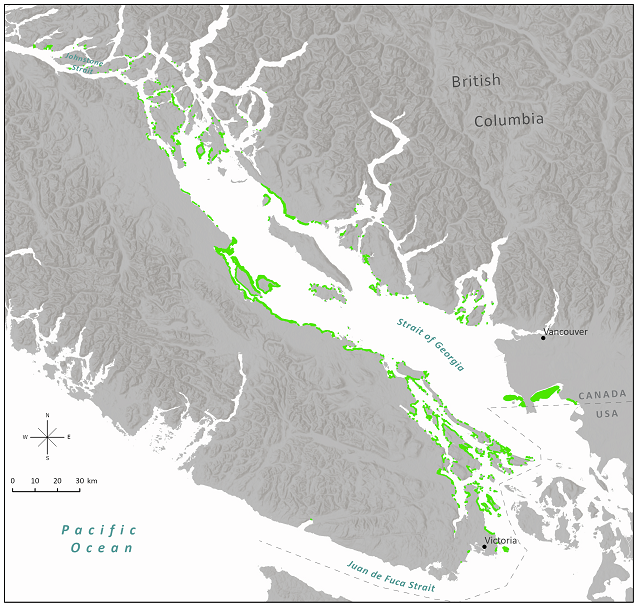
\includegraphics[width=6in]{figures/01_studyarea}}{Figure \ref{fig:studyareafig}} 

}

\caption{Study area. Finish caption on seagrass and bioregions.}\label{fig:studyareafig}
\end{figure}
\hypertarget{shoreline-area-adjacent-to-seagrass-meadows}{%
\subsection{Shoreline area adjacent to seagrass meadows}\label{shoreline-area-adjacent-to-seagrass-meadows}}

Past guidelines on the width of marine riparian buffer zones for protecting sensitive habitat typically range from 50-150 meters (\protect\hyperlink{ref-Levings2001}{Levings and Jamieson 2001}; \protect\hyperlink{ref-Lemieux2004}{Lemieux et al. 2004}). We followed the methodology in a similar study of anthropogenic impacts (\protect\hyperlink{ref-Iacarella2018}{Iacarella et al. 2018}) and examined shoreline modifications within 100 m of the coastline adjacent to each seagrass meadow. Quantifying modifications within a buffer zone requires generating consistent buffers from all meadows onto land. The perimeters of meadows, however, do not always exactly border the shoreline due to variable mapping accuracies and errors, as well as some meadows only existing in the subtidal zone. This results in slighlty different buffer extents on to land. Aside from a few exceptions, the majority of meadows are in close proximity to a coastline, and therefore, to create consistent width buffers on land we first adjusted the perimeter of meadows to match the coastline using digitization tools in ArcGIS.

\hypertarget{shoreline-modifications}{%
\subsection{Shoreline modifications}\label{shoreline-modifications}}

To quantify shoreline modification adjacent to seagrass, we identified any structures (e.g.~buildings, houses) and areas de-vegetated from their natural state (e.g.~lawns, logged areas, agriculture, armoured shoreline) within the 100 meter buffer. De-vegetated areas can increase nutrient run-off from agricultural areas and sewage outfalls potentially resulting in eutrophication (\protect\hyperlink{ref-hauxwell2003}{Hauxwell et al. 2003}; \protect\hyperlink{ref-vandermeulen2005}{Vandermeulen 2005}; \protect\hyperlink{ref-Quiros2017}{Quiros et al. 2017}). Hardened and de-vegated areas may also increase the outflow of sedimentation resulting in decreased light levels in seagrass meadows (\protect\hyperlink{ref-Vandermeulen2012}{Vandermeulen et al. 2012}; \protect\hyperlink{ref-Dethier2016}{Dethier et al. 2016}; \protect\hyperlink{ref-Todd2019}{Todd et al. 2019}).

Shoreline modifications were digitized from satellite and aerial imagery in Google Earth Pro. The most recent imagery available was used, but the dates of the imagery varied across the study area. The majority of roads were included using an existing provincial dataset (Province of British Columbia - Digital Road Atlas). This dataset consists of linear features which were buffered using the number of lanes and standard lane widths. Modifications were classified into six categories: road, residential, cropland, industrial, greenspace, unclear. Within each category, an additional descriptor was also listed (Table~\ref{tab:modifications}). Overwater structures (e.g.~floathomes, docks, aquaculture) were not considered to be shoreline modifications as these are associated with a different suite of impacts (e.g.~shading, boat traffic), and these features were captured in a separate study.

To quantify the overall level of shoreline modification we totaled the area of all modification types per buffered area and calculated the percent of the buffered area that is modified. The percent modified was then associated back with the adjacent seagrass meadow.
\begin{table}[h]

\caption{\label{tab:modifications}Shoreline modification classifications and descriptors}
\centering
\fontsize{9}{11}\selectfont
\begin{tabular}[t]{>{\centering\arraybackslash}m{10em}>{\raggedright\arraybackslash}m{30em}}
\toprule
\textbf{Modification} & \textbf{Subcategory descriptors}\\
\midrule
Road & paved; dirt; rail\\
\addlinespace
Residential & house; RV; lighthouse\\
\addlinespace
Industrial & logging; airport; general development; parking; storage; marina; church; electrical; ferry; hospital; train yard; shipping\\
\addlinespace
Cropland & crop; fishfarm\\
\addlinespace
Greenspace & cleared; campground; golf; park; recreation\\
\addlinespace
Unclear & unclear\\
\bottomrule
\end{tabular}
\end{table}
\hypertarget{results}{%
\section{Results}\label{results}}

The spatial distribution of shoreline modifications varied across the region. Examples of the extent and diversity of modifications are shown in Figure~\ref{fig:exampleareas}, and the full dataset is accessible online (see Data availability section). As expected, the seagrass meadows with the highest total levels of adjacent shoreline modification occurred near population centers (Figure~\ref{fig:percentmod}). The lowest levels of modification occurred near islands and in the northern part of the study area (i.e.~Johnstone Strait). The dominant modification type tended to vary by latitude. For example, there is more coastal agriculture in the south and more logging in the north (Figure ).

(\emph{TODO: make colors more bold in example figure.}) (\emph{TODO: add cities and towns to overall figure}) (\emph{TODO: do a full page figure for the 5 types. If these come after the total one, then I could try to fit them on one page.})
\begin{figure}[H]

{\centering \pdftooltip{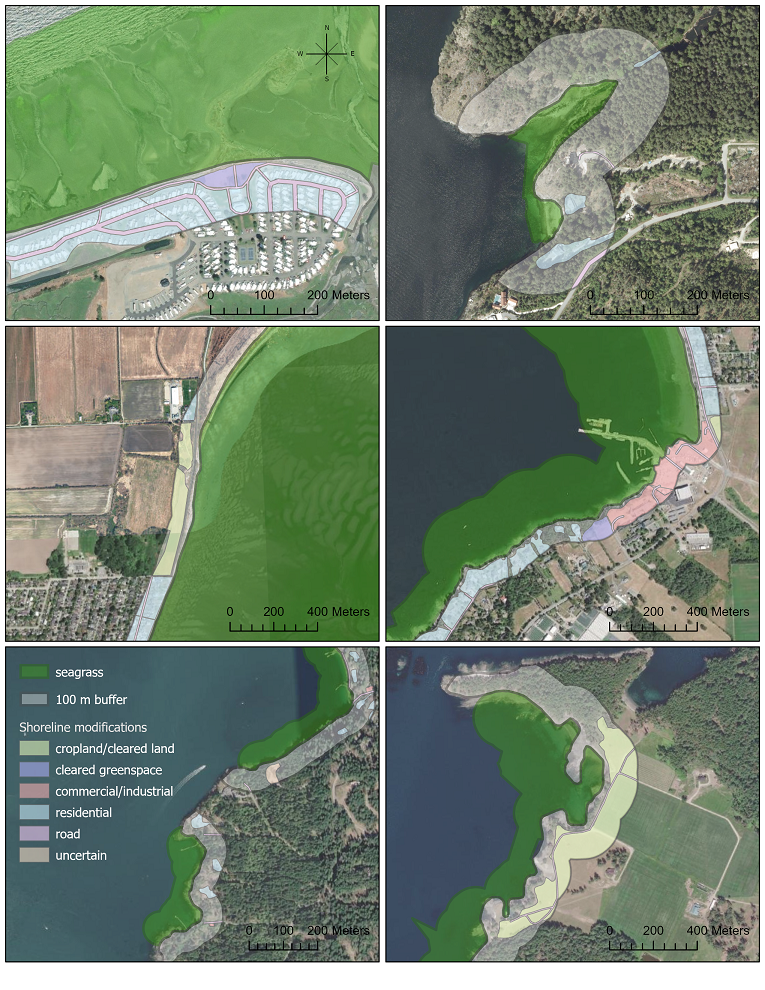
\includegraphics[width=6in]{figures/02_shorelinemod_examples}}{Figure \ref{fig:exampleareas}} 

}

\caption{Shoreline modifications within 100 meter buffered areas. The six selected areas are shown for example and do not imply any significance over other areas.}\label{fig:exampleareas}
\end{figure}
\begin{figure}[H]

{\centering \pdftooltip{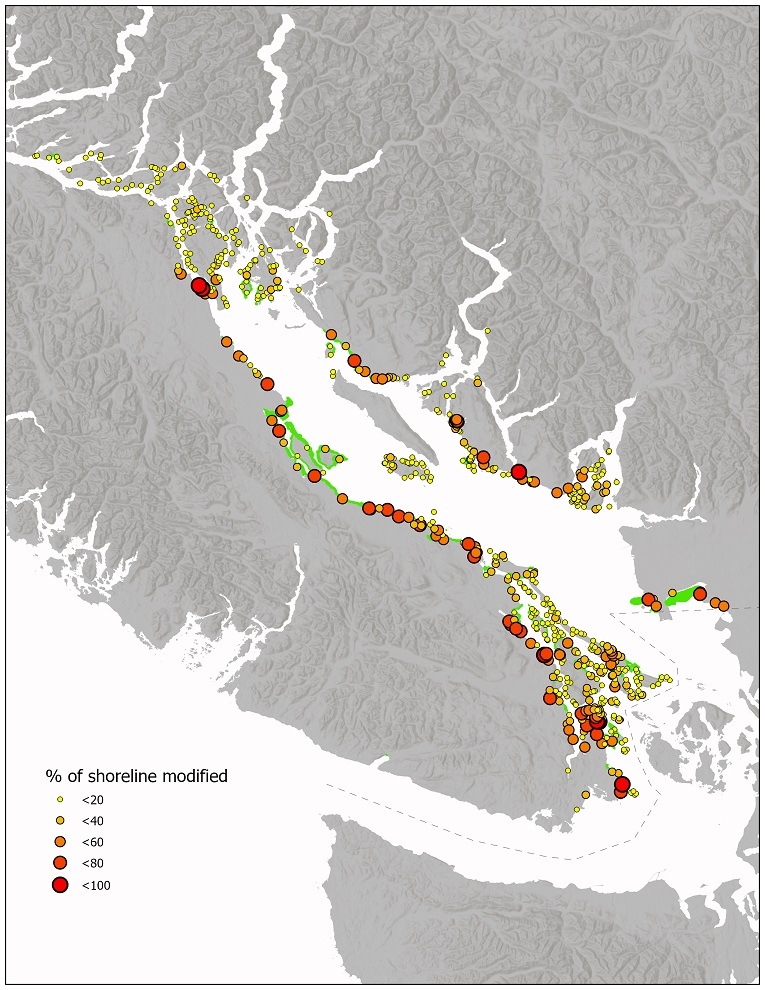
\includegraphics[width=6in]{figures/03_shorelinemod_percentage}}{Figure \ref{fig:percentmod}} 

}

\caption{The percentage of the shoreline buffered area that is modified.}\label{fig:percentmod}
\end{figure}
\hypertarget{discussion}{%
\section{Discussion}\label{discussion}}

(*first paragraph: summary sentences and some management goal stuff)

By quantifying shoreline modifications adjacent to seagrass meadows, we've provided a novel high resolution dataset for documenting land use over a large spatial extent and predicting potential impacts to nearshore ecosystems. The variation of the distribution and patterns of modifications across the region illustrate the different threats that seagrass meadows face based on their location. Few meadows had no adjacent modifications, but even then, shoreline modifications are only one type of activity that can threaten a seagrass meadow. If an area including a meadow is selected for management, then its likely the shoreline modifications will have to be considered, and the type of management action will vary with the type of modification. For example, limiting forestry activities vs.~managing activities on private land and managing the flow of sewage outflow. Consider management goals of protecting the most natural meadows and how this might change given the spatial distribution of activities and other information (e.g.~biodiversity in meadows, connectivity) See how Emily's EBSA paper discusses some of this.

(*2nd: vulnerability score variability) - This work can be incorporated into CI frameworks (e.g.~REFS) - incorporate vulnerability scores to specific types of modifications (cite CI research) - some stuff from my thesis: ``managing seagrass habitat and associated species in a landscape context, in which patterns of distribution, dispersal, and impacts will interact to influence regional management strategies (Murphy et al.~2021b). Although eelgrass is declining globally (Dunic et al.~2021), eelgrass in nearby Puget Sound, Washington is stable and resilient overall, despite a significant increase in local human and climactic stressors (Shelton et al.~2016). Assessing the relevance of managing for human impacts in the Salish Sea will therefore require a deeper understanding of seagrass and invertebrate responses to stressors and the mechanisms (e.g., dispersal) that allow for resilience to these stressors. Ultimately, refining and validating our models will increase their utility and promote their incorporation into broader marine spatial planning efforts.''

(*3rd: assumptions and limitations)

When using and adapting the data for future studies, certain assumptions need to be considered. - If the modification exists behind some vegetation then the impact could be less. - We use a uniform buffer, but there is a likely a distance decay for some of these activities. - No point measurements in field to confirm the severity of impacts of different modifications. Some activities are well regulated in Canada, like logging, and there may be very minimal impact. Whereas, drainage of waste and stormwater from seemingly well vegetated residential areas may have a high impact but hard measure. - Meadows that aren't right on the coast may not experience the same level of impacts as an intertidal meadow. - Ultimately, quantifying severity and vulnerability will increase the utility of this dataset for future marine spatial planning and management efforts. (should also work in to this idea something about this is connectivity terrestrial landscape features with seascape ecology.)

\hypertarget{data-availability}{%
\section{Data availability}\label{data-availability}}

Link to code in github repo Link to dataset wherever it gets hosted

\clearpage

\hypertarget{references}{%
\section{References}\label{references}}

\noindent \vspace{-2em} \setlength{\parindent}{-0.2in} \setlength{\leftskip}{0.2in} \setlength{\parskip}{8pt}

\hypertarget{refs}{}
\begin{CSLReferences}{1}{0}
\leavevmode{\hypertarget{ref-ClarkeMurray2015}{}}%
Clarke Murray, C., Agbayani, S., Alidina, H.M., and Ban, N.C. 2015. \link{https://doi.org/10.1016/j.marpol.2015.04.003}{Advancing marine cumulative effects mapping: {An} update in {Canada}'s {Pacific} waters}. Marine Policy 58: 71--77.

\leavevmode{\hypertarget{ref-Cristiani2021}{}}%
Cristiani, J., Rubidge, E., Forbes, C., Moore-Maley, B., and O'Connor, M.I. 2021. \link{https://doi.org/10.3389/fmars.2021.717469}{A {Biophysical Model} and {Network Analysis} of {Invertebrate Community Dispersal Reveals Regional Patterns} of {Seagrass Habitat Connectivity}}. Frontiers in Marine Science 8: 1--19.

\leavevmode{\hypertarget{ref-Dethier2016}{}}%
Dethier, M.N., Raymond, W.W., McBride, A.N., Toft, J.D., Cordell, J.R., Ogston, A.S., Heerhartz, S.M., and Berry, H.D. 2016. \link{https://doi.org/10.1016/j.ecss.2016.03.033}{Multiscale impacts of armoring on {Salish Sea} shorelines: {Evidence} for cumulative and threshold effects}. Estuarine, Coastal and Shelf Science 175: 106--117. {Elsevier Ltd}.

\leavevmode{\hypertarget{ref-DFO2019}{}}%
DFO. 2019. Design strategies for the {Northern Shelf Bioregion Marine Protected Area Network}. CSAS.

\leavevmode{\hypertarget{ref-Halpern2019}{}}%
Halpern, B.S., Frazier, M., Afflerbach, J., Lowndes, J.S., Micheli, F., O'NAHara, C., Scarborough, C., and Selko, K.A. 2019. \link{https://doi.org/10.1038/s41598-019-47201-9}{Recent pace of change in human impact on the world's ocean}. Scientific Reports 9(1): 1--8.

\leavevmode{\hypertarget{ref-hauxwell2003}{}}%
Hauxwell, J., Cebri'an, J., and Valiela, I. 2003. \link{https://doi.org/10.3354/meps247059}{Eelgrass {Zostera} marina loss in temperate estuaries: Relationship to land-derived nitrogen loads and effect of light limitation imposed by algae}. Mar. Ecol. Prog. Ser. 247: 59--73.

\leavevmode{\hypertarget{ref-Iacarella2018}{}}%
Iacarella, J.C., Adamczyk, E., Bowen, D., Chalifour, L., Eger, A., Heath, W., Helms, S., Hessing-Lewis, M., Hunt, B.P.V., MacInnis, A., O'Connor, M.I., Robinson, C.L.K., Yakimishyn, J., and Baum, J.K. 2018. \link{https://doi.org/10.1111/gcb.14090}{Anthropogenic disturbance homogenizes seagrass fish communities}. Global Change Biology 24(5): 1904--1918.

\leavevmode{\hypertarget{ref-Lemieux2004}{}}%
Lemieux, J.P., Brennan, J.S., Farrell, M., Levings, C.D., and Myers, D. 2004. {PROCEEDINGS OF THE DFO}/{PSAT SPONSORED MARINE RIPARIAN EXPERTS WORKSHOP}, {TSAWWASSEN}, {BC}, {FEBRUARY} 17-18, 2004.

\leavevmode{\hypertarget{ref-Levings2001}{}}%
Levings, C., and Jamieson, G. 2001. Marine and estuarine riparian habitats and their role in coastal ecosystems, {Pacific} region. Canadian Science Advisory Secretartiat: 41.

\leavevmode{\hypertarget{ref-Murphy2021a}{}}%
Murphy, G.E.P., Dunic, J.C., Adamczyk, E.M., Bittick, S.J., Côt'e, I.M., Cristiani, J., Geissinger, E.A., Gregory, R.S., Lotze, H.K., O'Connor, M.I., Ara'ujo, C.A.S., Rubidge, E.M., Templeman, N.D., and Wong, M.C. 2021. \link{https://doi.org/10.1139/facets-2020-0020}{From coast to coast to coast~: Ecology and management of seagrass ecosystems across {Canada}}. Facets 6: 1--41.

\leavevmode{\hypertarget{ref-Nagel2020}{}}%
Nagel, E.J., Murphy, G.E.P., Fast, J., Bittick, S.J., Adamczyk, M., Connor, M.I.O., Wong, M.C., and Lotze, H.K. 2020. Application of a coastal human impact metric and nitrogen loading model to 10 eelgrass ( {Zostera} marina ) meadows in {British Columbia}. {Fisheries and Oceans Canada}.

\leavevmode{\hypertarget{ref-Nahirnick2019}{}}%
Nahirnick, N.K., Costa, M., Schroeder, S., and Sharma, T. 2019. \link{https://doi.org/10.2112/jcoastres-d-18-00112.1}{Long-{Term Eelgrass Habitat Change} and {Associated Human Impacts} on the {West Coast} of {Canada}}. Journal of Coastal Research 36(1): 30.

\leavevmode{\hypertarget{ref-Quiros2017}{}}%
Quiros, T.E.A.L., Croll, D., Tershy, B., Fortes, M.D., and Raimondi, P. 2017. \link{https://doi.org/10.1016/j.biocon.2017.03.011}{Land use is a better predictor of tropical seagrass condition than marine protection}. Biological Conservation 209: 454--463. {The Authors}.

\leavevmode{\hypertarget{ref-Rubidge2020}{}}%
Rubidge, E., Jeffery, S., Gregr, E.J., Gale, K.S.P., and Frid, A. 2020. Assessment of nearshore features in the {Northern Shelf Bioregion} against criteria for determining {Ecologically} and {Biologically Significant Areas} ( {EBSAs} ). DFO Canadian Science Advisory Secretariat. {Canadian Science Advisory Secretariat}.

\leavevmode{\hypertarget{ref-Todd2019}{}}%
Todd, P.A., Heery, E.C., Loke, L.H.L., Thurstan, R.H., Kotze, D.J., and Swan, C. 2019. \link{https://doi.org/10.1111/oik.05946}{Towards an urban marine ecology: Characterizing the drivers, patterns and processes of marine ecosystems in coastal cities}. Oikos: 1215--1242.

\leavevmode{\hypertarget{ref-UNCBD2008}{}}%
UN CBD. 2008. Decision adopted by the conference of the parties to the convention on biological diversity at its ninth meeting. UNEP/CBD/COP/DEC/IX/20.

\leavevmode{\hypertarget{ref-vandermeulen2005}{}}%
Vandermeulen, H. 2005. Assessing {Marine Habitat Sensitivity}: {A} case study with eelgrass ({Zostera} marina {L}.) And kelps ({Laminaria}, {Macrocystis}). {DFO Canadian Science Advisory Secretariat, Fisheries and Oceans Canada}.

\leavevmode{\hypertarget{ref-Vandermeulen2012}{}}%
Vandermeulen, H., Surette, J., and Skinner, M.A. 2012. Responses of {Eelgrass} ({\emph{Zostera}}{ \emph{Marina} }{\emph{L}}{\emph{.}}) To stress. DFO Can. Sci. Advis. Sec. Res. Doc. 2011/095. vi + 43 p.

\end{CSLReferences}
\end{document}
